\section*{Nonnegative sparse coding as a modern variant of the efficient coding hypothesis}

\subsection*{\revise{Efficient coding}}

% \revise{\Acf{NSC} can be understood as a modern rendition of
% \textbf{efficient coding}.
\revise{The fundamental principle of \textbf{efficient coding}
is that a sensory system is
adjusted to the specific statistics of the natural environment from which
it encodes and transmits information
\cite{Barlow1961,Attneave1954,Linsker1990,LouieGlimcher2012}.}

Early theories of efficient coding
\cite{Barlow1961,Attneave1954}
were developed based on the visual system.
\revise{Attneave \cite{Attneave1954} pointed out that there is a significant
degree of redundancy in natural visual images due to correlations in both
the spatial and temporal domains
(for a recent review, see \cite{SimoncelliOlshausen2001}).
For example, the luminance values of a pair of pixels
separated by a fixed distance in a natural image
are likely to be highly correlated
(Fig.~\ref{fig:ech}A).
These statistical regularities constrain the images a visual system
is likely to encounter to a tiny fraction of the set of all
possible images.
It was therefore argued} that the visual system should not
waste resources on processing arbitrary images,
\revise{but instead} use statistical knowledge
about its environment to represent the relevant input space 
as economically as possible.


\begin{figure}[h]
	\centering
	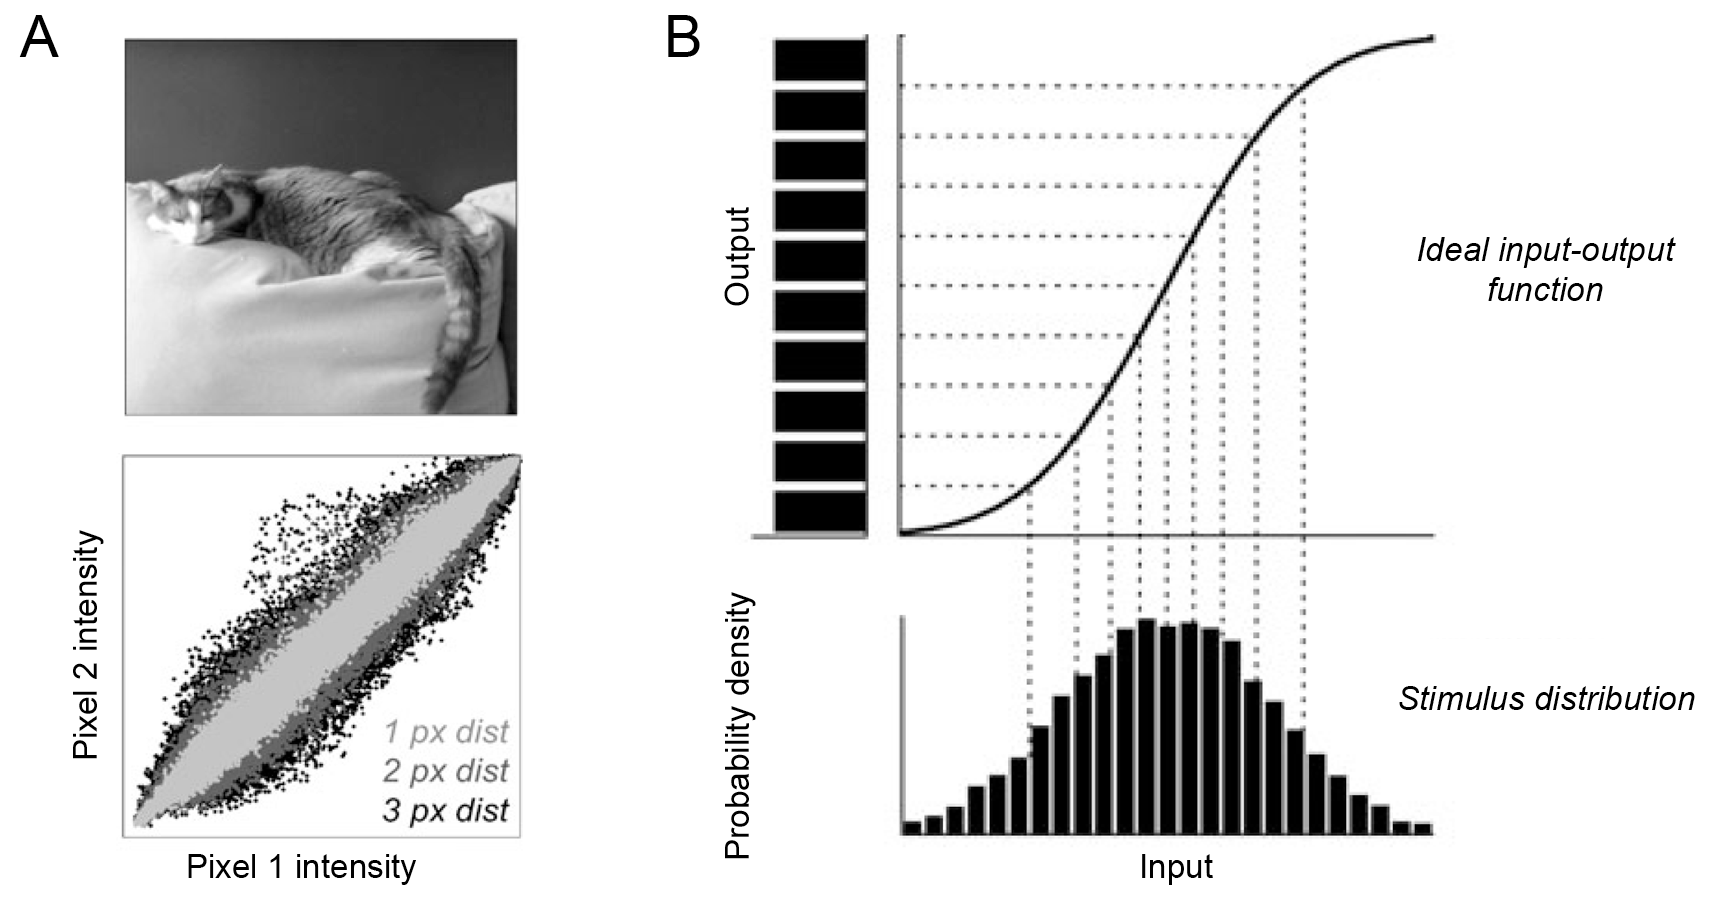
\includegraphics[width=\textwidth]{fig-rev1-ech}
    \caption{\revise{Efficient coding hypothesis
    	(reprinted from Louie \& Glimcher \cite{LouieGlimcher2012}).
    	A) Sensory stimuli in the environment, such as the image of the cat,
           display significant statistical structure. For example, the luminance
           value of nearby pixels in the image are significantly correlated,
           an effect that exists even for nonadjacent pixels.
           Neural systems can improve their coding efficiency by accounting
           for and reducing such information redundancy.
        B) For a given distribution of sensory characteristics in the world (bottom),
           an efficient neural input-output function produces an output (top)
           that equally uses all possible levels of neural activity.
    }}
	\label{fig:ech}
\end{figure}


\revise{Extending this idea to the neural level,
Barlow \cite{Barlow1961} proposed that
the goal of early neurons in sensory processing is to remove
the redundancy in the input stimuli.}
These \revise{ideas} were shaped by two
fundamental empirical observations
about early visual cortex:
1) a neuron's \ac{RF} resembled a decomposition of the visual
stimulus into a series of local, largely independent feature components
(e.g., a 2-D Gabor function is basically a local approximation of the
directional spatial derivative of an image),
and 2) any individual neuron responded only sparsely to a small subset of
stimulus features (e.g., orientation or color at a particular spatial location).
Thus a neuron's \ac{RF} could be understood as a
sparse, low-dimensional embedding of high-dimensional input stimuli.

\revise{At the level of single neurons, efficient coding requires
\mikeNote{These two blue paras are too close in wording to Louie and Glimcher - reword}
that the input-output function be adjusted so that the entire response
range is employed to represent the stimulus distribution \cite{Simoncelli2003}.
For example, under the constraints of a maximum firing rate and finite precision,
efficient neurons should employ all activity levels equally in response
to the distribution (Fig.~\ref{fig:ech}B).
If the input-output function sensitivity is too low,
high levels of the stimulus feature will be indistinguishable
as the response function saturates; if the sensitivity is set too high,
low levels of the stimulus feature cannot drive responses.}

\revise{When the activity of multiple neurons are considered together,
the efficient coding hypothesis requires that the joint encoding of
a stimulus should reflect both optimal responses in individual neurons
and efficiency across the set of neurons.
For example, to maximize efficiency and reduce redundancy, neural responses
should be independent of one another (decorrelated),
and a given stimulus should involve only a small fraction of the
available neurons (sparse) \cite{LouieGlimcher2012}.}


\subsection*{\revise{Nonnegative sparse coding}}

\revise{Taking these ideas a step further,}
Olshausen and Field \cite{OlshausenField1996} found that
linear sparse coding of natural images
yielded features qualitatively similar to
\acp{RF} of simple cells in \ac{V1},
thus giving empirically observed \acp{RF} an information-theoretic explanation.
However, as pointed out by Hoyer \cite{Hoyer2003}, sparse coding falls short
of providing a literal interpretation for \ac{V1} simple-cell behavior
for two reasons:
1) every neuron could be either positively or negatively active, and
2) the input to the neural network was typically double-signed,
whereas \ac{V1} neurons receive visual input from the \ac{LGN} 
in the form of separated, nonnegative ON and OFF channels.

Hoyer \cite{Hoyer2002,Hoyer2003} proposed \ac{NSC} as a way 
to transform Olshausen and Field's sparse coding 
from a relatively abstract model of image representation 
into a biologically plausible model of early visual cortex processing
by enforcing both input signal and neuronal activation to be nonnegative.
This seemingly simple change had remarkable consequences on the quality of the
sensory representation:
Whereas elementary image features in the standard sparse coding model could
`cancel each other out' through subtractive interactions,
enforcing nonnegativity ensured that features combined additively,
much like the intuitive notion of combining parts to form a whole.
The resulting parts-based representations resembled \acp{RF} in \ac{V1} 
much more closely than other holistic representations.

Inhibitory connections can be modeled in the same fashion,
by interpreting inhibitory weights as nonnegative synaptic conductances,
which not only
% Since neurons tend to release the same set of neurotransmitter at all of their
% terminals (Dale's principle), one would rarely have to use both excitatory and inhibitory weights
% Mixing of excitatory and inhibitory weights \emph{within a particular pre-post connection} 
% is rare, since neurons tend to release a single kind or class of neurotransmitters
% (Dale's principle).
% This is consistent with Dale's principle, which states that neurons
% tend to release a single kind or class of neurotransmitters.
% Modeling all synaptic weights as nonnegative synaptic conductances not only
preserves the parts-based quality of the encoding,
but also allows for more complicated connection types to be modeled
(e.g., \ac{V1} neurons receiving input from both excitatory ON
and inhibitory OFF cells in the \ac{LGN})
\cite{Hoyer2003}.
However, it is interesting to note that a more recent study has argued
that the nonnegativity constraint on the
synaptic weights might not be necessary to preserve the parts-based quality of
the encoding \cite{Liu2017}.


\Ac{NSC} combines \ac{NMF}, a linear dimensionality reduction technique from statistical learning, with sparse population coding from neural network theory \cite{Hoyer2002,EggertKorner2004}.
\Ac{NMF} belongs to a class of methods that can be used to decompose multivariate data matrix \textbf{V} into an inner product of two reduced-rank matrices \textbf{W} and \textbf{H}, such that $\mathbf{V} \approx \mathbf{WH}$. \Ac{NMF} assumes that the observed data in \textbf{V} are caused by a collection of \revise{hidden variables}
weighted by nonnegative numbers, representing both their presence and intensity.

In the context of \ac{NSC},
\mikeNote{You know, this stuff would be so much clearer if we had a figure. It's kinda silly not to have a figure for the main algorithm. I'm picturing the NMF schematic from Fig.3 together with Fig.4A that shows how to go from \textbf{W} in NMF all the way to neuronal responses $r_bs$.}
\textbf{V} and \textbf{H} correspond to activation values
of two distinct neuronal populations,
which are connected to each other via synaptic weight values
in \textbf{W}.
Consider a number of data samples $s \in [1, S]$, for example,
in the form of observed firing rates of a population of $F$ neurons.
If we arrange the observed values of the $s$-th observation 
into a vector $\vec{v}_s$,
and if we arrange all vectors into the columns of a data matrix \textbf{V},
then linear decompositions describe these data as
$\mathbf{V} \approx \mathbf{WH}$.
Here, \textbf{W} is a matrix that contains as its columns
a total of $B$ \emph{basis vectors} of the decomposition, 
\mikeNote{Scale back the jargon}
and \textbf{H} contains as its rows the \emph{hidden coefficients}
that give the contribution of each basis vector in the input vectors.
The difference between \textbf{V} and \textbf{WH} is termed
the \emph{reconstruction error}.

The goal of \ac{NSC} is then to find a linear decomposition of \textbf{V}
that minimizes the reconstruction error,
while guaranteeing that both \textbf{W} and \textbf{H} are sparse.
This can be achieved by minimizing the following cost function
\cite{Hoyer2002}:
\begin{equation}
\min_{\mathbf{W}, \mathbf{H}} \frac{1}{2} ||\mathbf{V} -\mathbf{WH}||^2 + \lambda \sum_{ij} f(\mathbf{H}_{ij}),
\end{equation}
subject to the constraints
$\forall ij: \mathbf{W}_{ij} \geq 0$, $\mathbf{H}_{ij} \geq 0$, and
$||\vec{w}_i|| = 1$, where $\vec{w}_i$ denotes the $i$-th column of \textbf{W}.
Here, the left-hand term describes the reconstruction error, which can
be minimized with \ac{NMF}
(typically done using alternating least-squares techniques),
and the right-hand term describes the sparsity of the decomposition.
The trade-off between sparsity and accurate reconstruction
is controlled by the parameter $\lambda$ ($\lambda \geq 0$), whereas
the form of $f$ defines how sparsity is measured
(a typical choice is the L1 norm on \textbf{H}).
Another open parameter is the number of basis vectors, $B$, which controls the sparsity of the embedding (see \cite{Beyeler2016}) and has to be
determined empirically.


